\documentclass[12pt]{scrartcl}

\usepackage[utf8]{inputenc}
\usepackage[naustrian]{babel}
\usepackage{caption}
\usepackage{graphicx}
\usepackage{verbatim}
\usepackage[T1]{fontenc}
\usepackage{lmodern}
\usepackage{subcaption}
\usepackage{amsfonts}
\usepackage{listings}
\usepackage{float}

%pdfs
\usepackage{pdfpages}
\usepackage{tikz}

%page borders
\usepackage{geometry}
\geometry{left=2.5cm,right=2.5cm,top=3cm,bottom=2.5cm}

\usepackage{minted}
\setminted {
	%style=igor, %borland, autumn, vs
	encoding=utf-8,
	autogobble,
	tabsize=4,
	linenos,
	breaklines,
	keywordcase=upper,
	%escapeinside=||
	%bgcolor=bg
	%frame=single
}

\newenvironment{code}{\captionsetup{type=listing}}{}

%title/footer/header values
\usepackage{titling}
\title{DES3UE Übung 4}
\author{Elias Leonhardsberger}
\date{\today{}, Hagenberg}

%footer/header
%\usepackage[automark]{scrpage2}
%\pagestyle{headings}
%\clearscrheadfoot
%\ihead{\thetitle}
%\chead{\theauthor}
%\ohead{\today}
%\cfoot{Seite \pagemark}

\begin{document}
\clearpage
\thispagestyle{empty}
\begin{tikzpicture}[remember picture, overlay]
	\node at (current page.center) {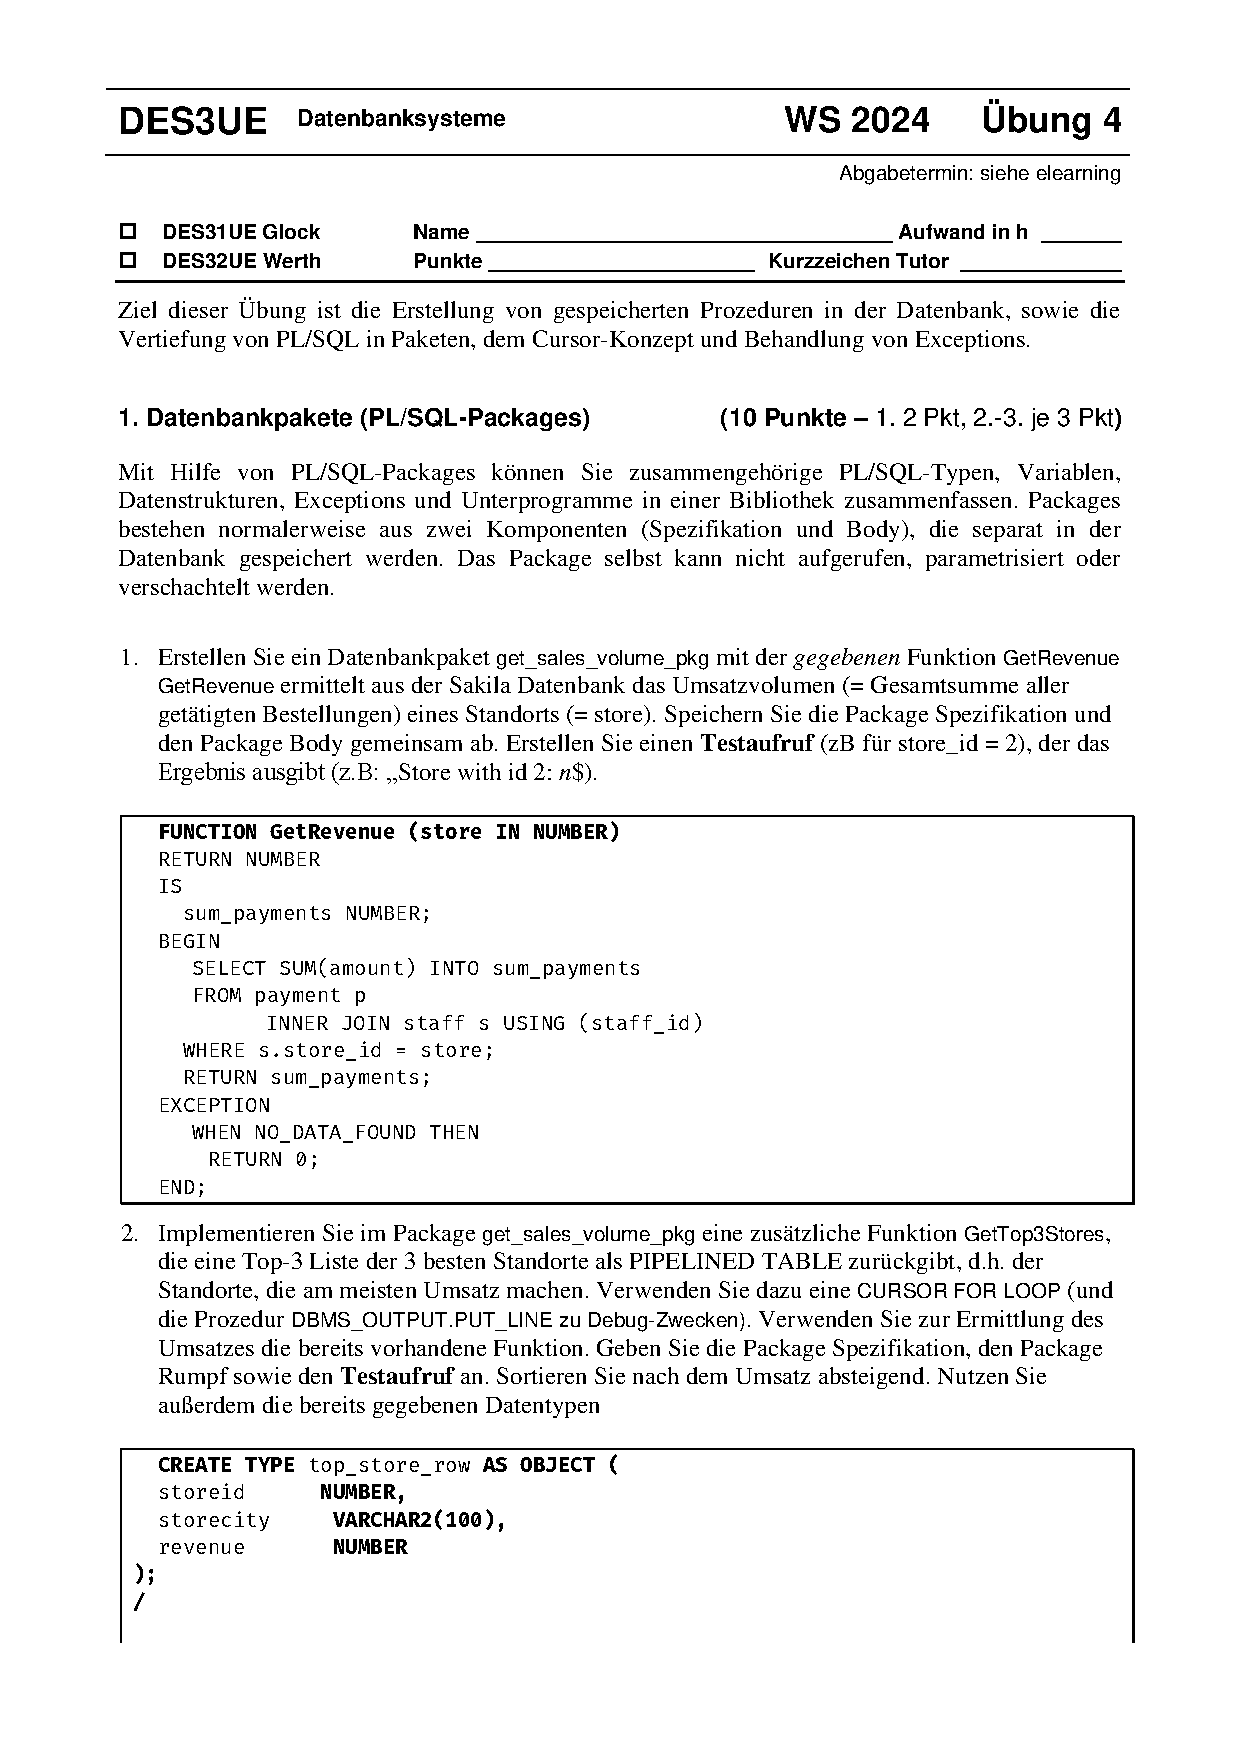
\includegraphics[page=1]{Angabe.pdf}};
	\begin{scope}[shift={(current page.south west)},every node/.style={anchor=base west}]
		\node at (1.87cm, 25.65cm) {X};
		\node at (8.5cm, 25.75cm) {\theauthor};
		\node at (17.7cm, 25.75cm) {3.5};
	\end{scope}
\end{tikzpicture}

\includepdf[pages=2-3]{Angabe.pdf}

\maketitle
\tableofcontents

\pagebreak

\section{Datenbankpakete (PL/SQL-Packages)}

\subsection{SQL}
\inputminted{sql}{../ue4_1.sql}

\subsection{Ergebnisse}
\begin{figure}[h]
	\centering
	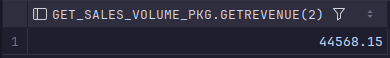
\includegraphics[width=0.8\textwidth]{../ue4_1_1.png}
	\caption{Ergebnis Aufgabe 1.1}
\end{figure}

\begin{figure}[h]
	\centering
	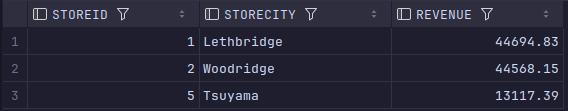
\includegraphics[width=0.8\textwidth]{../ue4_1_2.png}
	\caption{Ergebnis Aufgabe 1.2}
\end{figure}

\begin{figure}[h]
	\centering
	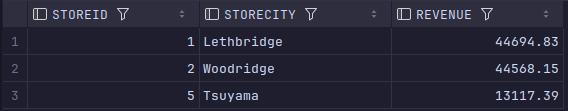
\includegraphics[width=0.8\textwidth]{../ue4_1_3.png}
	\caption{Ergebnis 1 Aufgabe 1.3}
\end{figure}

\begin{figure}[h]
	\centering
	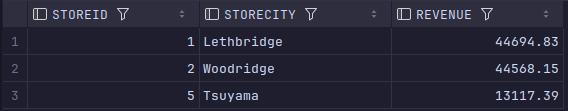
\includegraphics[width=0.8\textwidth]{../ue4_1_3.png}
	\caption{Ergebnis 2 Aufgabe 1.3}
\end{figure}

\pagebreak

\section{PL/SQL Prozeduren}

\subsection{SQL}
\inputminted{sql}{../ue4_2.sql}

\subsection{Ergebnisse}
\begin{figure}[h]
	\centering
	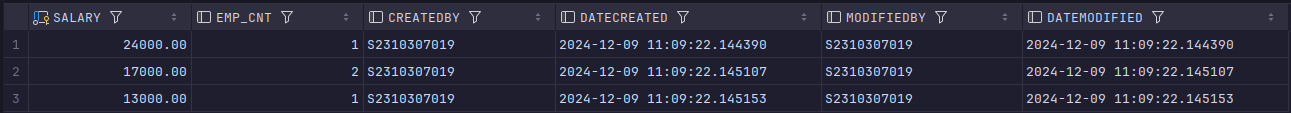
\includegraphics[width=1\textwidth]{../ue4_2.png}
	\caption{Ergebnis Aufgabe 2}
\end{figure}

\section{Cursor mit FOR-UPDATE}

\subsection{SQL}
\inputminted{sql}{../ue4_3.sql}

Für Aufgabe 3.3 und 3.4 wurde folgendes SQL-Statement verwendet:

\inputminted{sql}{../ue4_3_3.sql}

\pagebreak

\subsection{Ergebnisse}
\begin{figure}[h]
	\centering
	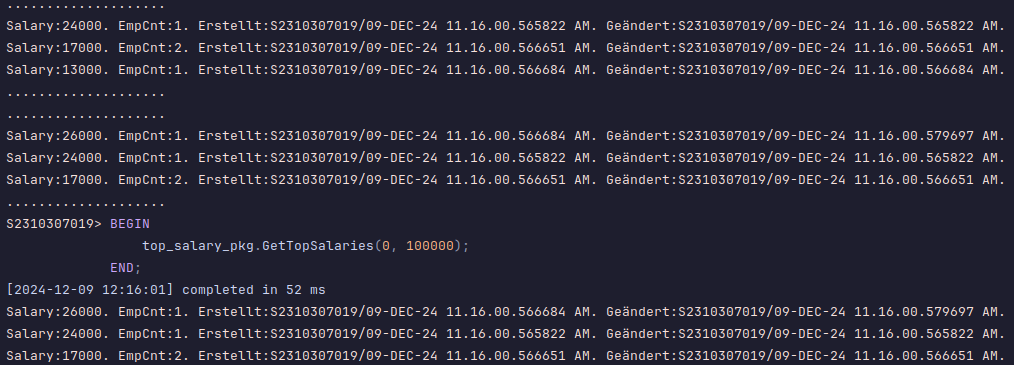
\includegraphics[width=1\textwidth]{../ue4_3_1.png}
	\caption{Ergebnis Aufgabe 3.1-3.2}
\end{figure}

\subsubsection{Ohne NOWAIT und COMMIT}

Die erste Session läuft durch, die anderen warten, bis die Transaktion der ersten Session beendet ist, also in dem Beispiel für immer.

\begin{figure}[h]
	\centering
	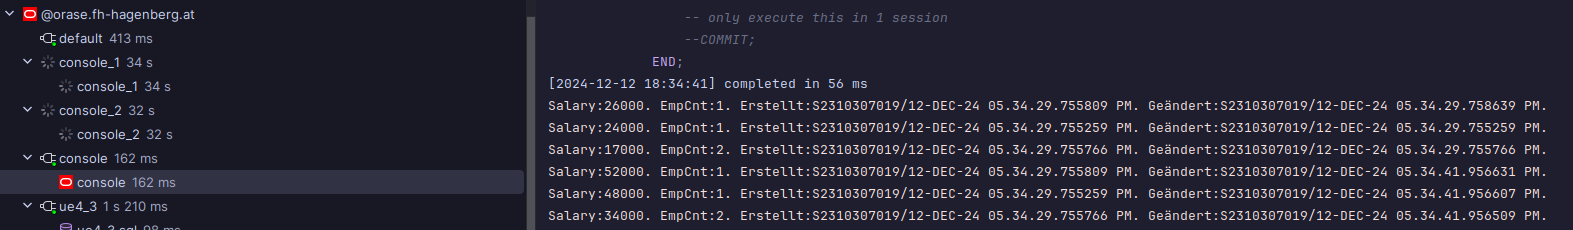
\includegraphics[width=1\textwidth]{../ue4_3_session1_1.png}
	\caption{Ergebnis Aufgabe 3.3 ohne COMMIT}
\end{figure}

\subsubsection{Ohne NOWAIT, mit COMMIT}

Da die Transaktion der ersten Session beendet ist, kann die zweite Session die Transaktion durchführen.

\begin{figure}[h]
	\centering
	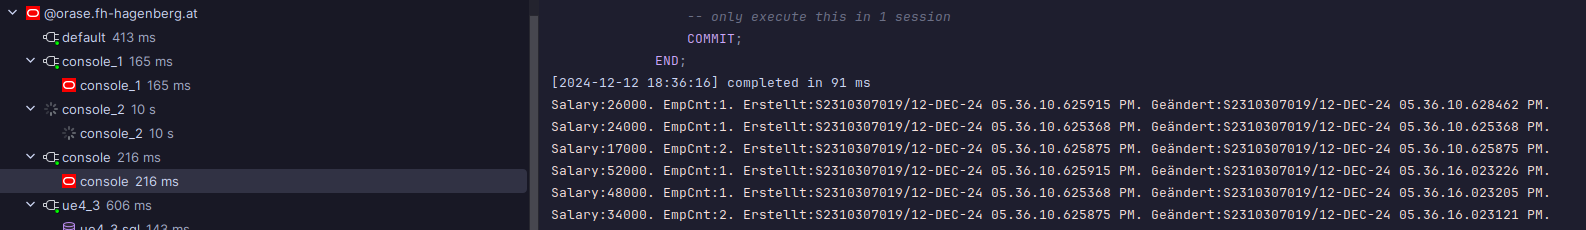
\includegraphics[width=1\textwidth]{../ue4_3_session1_2.png}
	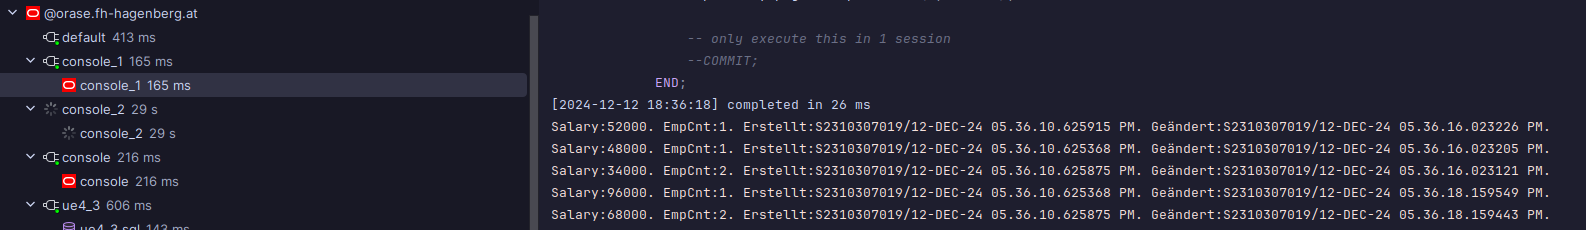
\includegraphics[width=1\textwidth]{../ue4_3_session2_1.png}
	\caption{Ergebnis Aufgabe 3.3 mit COMMIT}
\end{figure}

\pagebreak

\subsubsection{Mit NOWAIT}

Die erste Session führt einen Commit aus, dadurch ist die Transaktion beendet und die zweite Session läuft weiterhin problemlos durch.
Die dritte Session wartet aber jetzt nicht mehr, sondern gibt eine Fehlermeldung aus.

\begin{figure}[h]
	\centering
	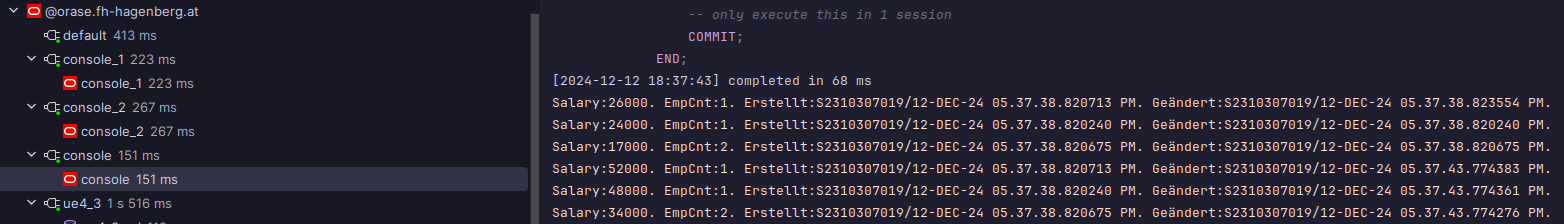
\includegraphics[width=1\textwidth]{../ue4_3_session1_3.png}
	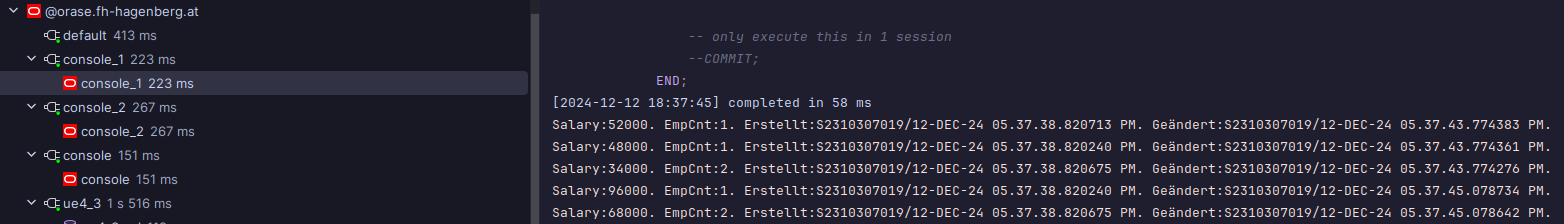
\includegraphics[width=1\textwidth]{../ue4_3_session2_2.png}
	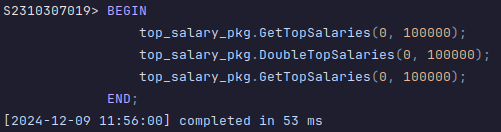
\includegraphics[width=1\textwidth]{../ue4_3_session3_1.png}
	\caption{Ergebnis Aufgabe 3.4}
\end{figure}
\end{document}